
\section{Background}
\label{sec:background}

In this section, we describe the anatomy of a simple email
transmission and the protocols used to authenticate such an email.
We also present a high-level overview of how forwarding modifies the
email delivery flow as a basis for a detailed description of
different forwarding approaches and implementations in
Section~\ref{sec:measure_forwarding_mechs_and_arc}.  Finally, we
briefly survey related work on email security, particularly
those whose insights we have built upon.
% In the remainder of the paper, we explore email forwarding in more depth and show how the inherent conflict between the functional goals of forwarding and anti-spoofing mechanisms enable a wide range of spoofing attacks.
% We then describe the range of forwarding mechanisms in use and how
% these create challenges for existing authentication protocols.

\subsection{Simple Mail Transfer Protocol}
The Simple Mail Transfer Protocol (SMTP) governs the addressing and
delivery of Internet email~\cite{rfc5321}.  Designed to mimic physical
mail, SMTP specifies two distinct sets of headers that declare the
sender and recipient(s) of an email message.  An outer set of headers,
the \emph{SMTP Envelope Headers} (\textsc{MAIL FROM} and \textsc{RCPT
  TO}), tell email servers how to route and deliver email. In
particular, the \textsc{RCPT TO} header identifies the message's
recipient and the \textsc{MAIL FROM} header identifies where to send
replies and bounce messages.  An inner set of headers, the
\emph{Message Headers} (\textsc{FROM} and \textsc{TO}), are contained
in the body of the SMTP message~\cite{rfc5322}.  These correspond to the
human-readable names and addresses set by email clients when the
sending user creates an email message.  These headers are strictly
intended for human user-interface purposes (\ie, for populating the
``To:'' and ``From:'' fields in email clients) and they are not used
for email routing.  Figure~\ref{fig:mech_smtp_headers} illustrates an
example message with both sets of headers.  Note that, although the
addresses in the Envelope and Message headers frequently match (as
they do in our example), they are not required to do so and there are both
benign (\eg, email forwarding) and malicious (\eg, phishing) reasons
for producing mismatched headers (\eg, where the \textsc{MAIL FROM}
address does not match the \textsc{FROM} address).
% the basic addressing of
% Internet email, via message fields and headers, as well as the online protocol
% for message addressing and transmission~\cite{rfc5321}.
% An important feature of SMTP is that it supports
% email transport across multiple networks. Thus, a email may pass through a
% number of intermediary forwarders on its path from sender to ultimate recipient.
% While SMTP specifies many aspects of the email transmission, relevant to our
% discussion are the SMTP email headers transmitted alongside the email body.
% An example of such an email message is depicted in
% Figure~\ref{fig:mech_smtp_headers}.  Notably, the notion of
% ``identity'' is aliased between the headers derived from the ``SMTP
% envelope'' created during an SMTP transaction and in the message's
% headers, created by Mail User Agent (MUA) software.  Thus, both
% the \textsc{MAIL FROM} and \textsc{FROM} headers identify the sender
% of a message and both the \textsc{RCPT TO} and \textsc{TO} headers
% identify the intended recipient.  However, they are not constrained to
% be the same and most MUA software will only display the message header
% fields when presenting mail to the user.

%via message headers,
%SMTP allows multiple ``identities'' for both the sender and
%receiver. For example, both the \texttt{MAIL FROM} and \texttt{FROM}
%headers identify the sender, but the former represents the identified
%sender transmitting the message via SMTP (and is generally not visible
%to the recipient) while the latter is part of the email message header
%and \emph{is} displayed to the recipient.\footnote{SMTP itself also
%  manages additional sending party identities, such as the HELO in
%  Figure~\ref{fig:mech_smtp_headers}, but we consider them
%  out-of-scope.} Similarly, both \texttt{RCPT TO} and \texttt{TO}
%headers identify the recipient --- respectively capturing the
%recipient identified in an SMTP transaction and the recipient
%identified in the message header (and displayed to the user).  These
%aliased fields do not need to be the same.


%\gakiwate{@@Alex: Check for correctness}

% \gakiwate{I nuked the discussion of the simple email transmission since we
% repeat it again in the email forwarding scenario. The discussion around POP/IMAP
% is not needed since we do not ever discuss it later.}

\begin{figure}[t]
    \centerline{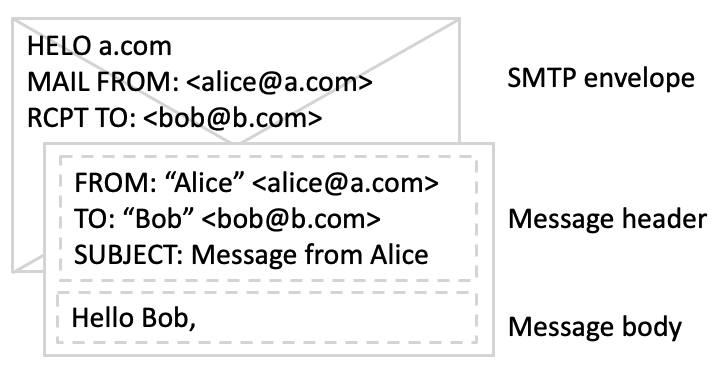
\includegraphics[width=\columnwidth]{fig/mech_smtp_headers.pdf}}
    \centering
    \caption[Example SMTP Headers]{Example SMTP headers in a transmission (inspired by Figure 3 in Chen et al.~\cite{chen2020composition}).}
    \label{fig:mech_smtp_headers}
\end{figure}

\subsection{Email Spoofing Protections}
The original SMTP design lacks authentication, which
has made email spoofing attacks both possible and common. To mitigate these attacks, the community has proposed multiple mechanisms that focus on authenticating the \emph{domain name} used by the
purported sender.\footnote{True per-sender authentication has long floundered
  due to the lack of effective mechanisms for binding user identities
  with cryptographic credentials at scale.  The best known protocol in
  this space, PGP, has been riddled with security and usability issues
  and remains, at best, a niche protocol.  In this paper, we focus
  exclusively on domain-level sender authentication.} Of these
mechanisms, we focus on SPF~\cite{rfc7208}, DKIM~\cite{rfc6376}, and DMARC~\cite{rfc7489} given their wide adoption.

%\subsubsection{SPF}
\medskip
\noindent\textbf{Sender Policy Framework (SPF)} defines a list of IP addresses permitted to send email on behalf of a domain and a set of actions the recipient should take if they receive an email from an unauthorized IP address.\footnote{In addition to lists of raw IP addresses, SPF
records can also ``include'' other SPF records by reference.}
Domain owners specify this policy by publishing it in a DNS TXT record.
Upon receiving an email message, the receiver fetches the list of authorized sender IP addresses by querying the domain in the email's \textsc{MAIL FROM} header.
The recipient then verifies if the IP address of the sending server is included that list.
If the verification fails, the receiver enforces the action (e.g., marking the email as spam) specified by the \textsc{MAIL FROM} domain in their SPF policy.


% When receiving email from a given IP address, a mail server queries the
% domain present in the \textsc{MAIL FROM} header to obtain its SPF
% policy (encoded in DNS TXT records) and checks whether the policy's list of allowed IP addresses includes the sending server's IP address.
% If the check fails, the mail server then enforces the filtering policy
% specified by the domain owner's SPF policy (\eg, hard fail, soft fail).
% \footnote{Note, it is recommended but not required to also
  % check against the domain identified in SMTP's HELO handshake.}
%
% One major problem with SPF is that it is not compatible with simple
% forwarding. When an email is forwarded, SPF checks can fail because a
% mail server will authenticate the forwarding server, rather than the
% original sending server.

%\subsubsection{DKIM}
\medskip
\noindent\textbf{DomainKeys Identified Mail (DKIM)} cryptographically
binds an email message with its sending email domain.  With DKIM, the
sender signs an email (or certain elements of an email) and attaches a digital signature via a
\textsc{DKIM-Signature} message header for future verification.
Receivers later retrieve the signer's public key (in the form of a DNS TXT record) from the domain specified in the \textsc{DKIM-Signature} header and authenticate an email's signature using that key.

Sadly, neither SPF nor DKIM verify that an email's purported sender (\ie, the \textsc{FROM} header) truly wrote and sent it~\cite{chen2020composition}.
For example, an attacker could bypass DKIM by spoofing an email's \textsc{FROM} header, but then sign and attach a DKIM signature that uses key pairs linked to their own domain (since DKIM does not compare the signature's domain against the \textsc{FROM} domain).
Attacks that exploit
this lack of \textsc{FROM} header authentication motivated the creation of DMARC.
% the \textsc{FROM} header
% displayed to the users, and passing SPF and/or DKIM validation does
% not guarantee the authenticity of the \textsc{FROM} header.  This
% lack, among other reasons, led to the creation of DMARC.

%\subsubsection{DMARC}
\medskip
\noindent\textbf{Domain Message Authentication, Reporting, and
Conformance (DMARC)} combines and extends SPF and DKIM to mitigate these security issues.
% authenticate the domain specified in the \textsc{FROM} header. 
Under DMARC, an email's receiver performs an ``alignment test'': checking if the
domain in the \textsc{FROM} header matches the domain name verified by
either SPF (the domain in the \textsc{MAIL FROM} header) or DKIM (the
domain in the \textsc{DKIM-Signature} header).
By default (``relaxed mode''), the alignment test only requires that the registered domains in the headers match (\ie, not the fully qualified domain name (FQDN)). However, domain owners can specify that recipients should follow the strict mode of the alignment test, which requires the \textsc{FROM} header's FQDN to exactly match the domain authenticated by SPF or DKIM.\footnote{%As with SPF, 
DMARC policy records are also stored as DNS TXT records.} 

If the email passes either SPF or DKIM authentication, and the alignment test also passes, then DMARC considers the email authenticated.
% The alignment test, and overall DMARC authentication for an email, succeeds if 
% The alignment test succeeds if the email passes under either the SPF or DKIM comparison
% When either SPF or DKIM are successful and the alignment test is also successful, the email is considered passing DMARC authentication.
Otherwise, the receiver should implement the DMARC policy designated by the domain in the \textsc{FROM} header, selected from one of three options: \textsc{None},
\textsc{Quarantine}, or \textsc{Reject}.  A policy of \textsc{None}
specifies that an email should be delivered as normal (and thus is often used for monitoring purposes~\cite{DMARCMonitoring1,DMARCMonitoring2}), and \textsc{Reject}
specifies that the recipient mail server should drop the email without
delivering it to the user.  The \textsc{Quarantine} policy is not strictly
defined (indicating only that the message should be treated ``as
suspicious'') and allows each email provider considerable latitude in
their implementation (\eg, setting a UI indicator or placing the email
in a designated spam folder)~\cite{rfc7489}.

%\subsubsection{UI-level Protection}
%% \paragraph{UI Indicators}
%% The combination of these various measures does
%% not always produce a clear binary signal.
%% Thus, email services frequently combine filtering rules with application-layer user interface (UI) indicators to help alert users when the authenticity of an email is suspect.
%% However, currently there is no standard for how and when such
%% UI indicators should be implemented, and different providers favor
%% different approaches.
%% \grant{I think we can completely cut this paragraph if we need space (IV.D.2 gives enough context about UI defenses without this.)}
%% \geoff{looking at IV.D.2, agreed}
% \grant{This part is a little thin, and might be worth folding into the
% vulnerability/attack section where relevant.}\amirian{agreed; it seems out of
% place here. unless this specifically comes into play in the attack section I
% would consider removing it}

% So, in addition to mandatory
% filtering rules, application-layer user interface (UI) indicators are also
% commonly used to help alert users when the authenticity of an email is
% suspect. However, currently there is no standard on how and when such
% UI indicators should be implemented, and different providers favor
% different approaches.

% (1) {\bf
% p=reject} the mail server rejects the email (2) {\bf p=quarantine} the mail
% server accepts the email but marks it as suspicious\gakiwate{Put it in Trash?}
% (3) {\bf p=none} the mail server accepts the email
% nevertheless.\gakiwate{@@Alex: spell out the DMARC policies and expected behavior}

% The DMARC policy None is the weakest and allows for spoofing since an email
% maybe accepted regardless of whether it passes SPF or DKIM. That said, most
% email providers will label such emails as suspicious and display warnings.
% Thus, even though a domain may have DMARC policy None an attacker still may
% have to defeat email providers' protections to deliver an email to the users
% inbox.

% \gakiwate{@@Alex: Make consistent with dmarc policy usage elsewhere.}

% Together these mechanisms can help authenticate emails and thus prevent the
% email spoofing.
%Next, we consider email forwarding and how it complicates these
%email authentication mechanisms.

\begin{figure}[t]
%  \vspace*{-0.2in}
\centerline{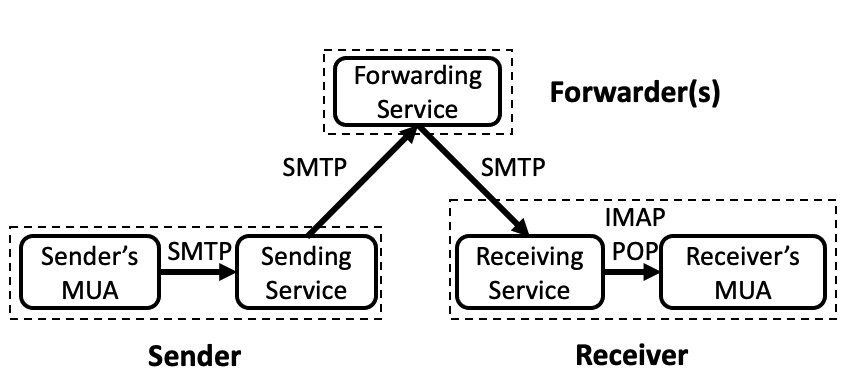
\includegraphics[width=\columnwidth]{fig/mech_email_forwarding_flow.pdf}}
\caption[Email Flow Involving Forwarding]{Email flow involving forwarding.}
\label{fig:email_forwarding_flow}
  \vspace*{-0.1in}
\end{figure}


\subsection{Email Forwarding}
\label{sec:background:fwd:overview}
% \amirian{can you give a one sentence example of a e.g. of a forwarder? someone
% who isnt familiar with forwarders might not understand who can run them and it
% would help to cement the understanding here}
Forwarding is ubiquitous in the email ecosystem and is necessitated by
the wide use of mailing lists~\cite{Electron8:online}, email filtering
services such as ProofPoint~\cite{SecureEm78:online}, and
auto-forwarding employed by individual users for account
aggregation~\cite{TheBestW9:online}, among others.  As shown in
Figure~\ref{fig:email_forwarding_flow}, forwarding alters the standard
transmission flow of an email message.  Instead of a direct
transmission from the sender to the recipient, forwarding relays an
email from the sender to an intermediate server and/or account, which
then transmits a copy of the email to the final recipient.
% (e.g., when a student configures her university email account to forward all messages to a pre-existing personal email address).
For simplicity we show a single forwarder in our example, but email can pass through multiple forwarders in common use cases. % (note, while the figure shows a single forwarder, it is possible to have multiple such forwarders in series).
%While Figure~\ref{fig:email_forwarding_flow}
%shows a single forwarder it is possible to have multiple forwarders.
%Additionally, a forwarder may not always have a domain name associated with it.
%\gakiwate{@@Alex: ProofPoint does not have a domain name no? Check.}

% Forwarders play the same role as receivers but also seek to
% retransmit the original message to a new destination.
Like normal receivers in direct mail transfer,
forwarders are responsible for performing standard authentication checks on each email they receive. % as normally done by a receiver.
However, after authenticating a message,
a forwarder often makes \emph{changes} to the email headers and/or the
email body based on the service it provides.
%(\S~\ref{sec:measure_forwarding_mechs_and_arc}).
The forwarder then sends the modified message to the final receiver (or next forwarder), which also performs authentication checks upon receiving the email.
Finally, when a recipient receives and opens an email, the receiver's user agent (MUA) parses and displays the message to the user.
%If such an email fails DMARC authentication checks at the receiver, the receiver should follow the DMARC policy specified in the email's \texttt{FROM} header.
% Finally, an email is parsed and displayed at the recipient's mail user
% agent.

%. Additionally, most email providers add their own
%warnings if needed based on the email. While an email contains
%multiple headers that represent different sender identities, the MUA
%generally only displays the FROM header and optionally displays other
%headers~\cite{chen2020composition}.
%
% However, the need to accommodate email forwarding while reliably
% authenticating emails introduces challenges. For example, SPF
% validation frequently fails because the receiver will attempt to
% authenticate the forwarding service (which frequently does not have
% the same domain as the \textsc{MAIL FROM} header) rather than the
% original sending server.  Moreover, DKIM checks may fail if a
% forwarder modifies the email body (\eg, many mail filtering services
% rewrite URLs in the email body to offer post-delivery protection). The
% resulting DMARC failures may thus prevent forwarded mail from being
% delivered (\ie, if the \textsc{FROM} domain DMARC policy is quarantine or
% reject).  To prevent this outcome, and preserve the utility of
% forwarders, forwarding services modify email headers to try to ensure
% email delivery. Unfortunately, there is no accepted standard for these
% modifications and different providers use different strategies ---
% \emph{forwarding mechanisms} --- to forward email.  We describe four
% such forwarding mechanisms
% (Figure~\ref{fig:forwarding_mechs_combined}) that are relevant to this
% paper. While some mechanisms are well-documented (\eg, remailing),
% others are ad-hoc and not as well-documented.

%while others are custom and less well-documented \alex{e.g. MAIL FROM equals
%FROM, which is used by outlook}.

% %\subsubsection{Email Forwarding Mechanisms}
% \begin{figure}[t]
%     \centering
%     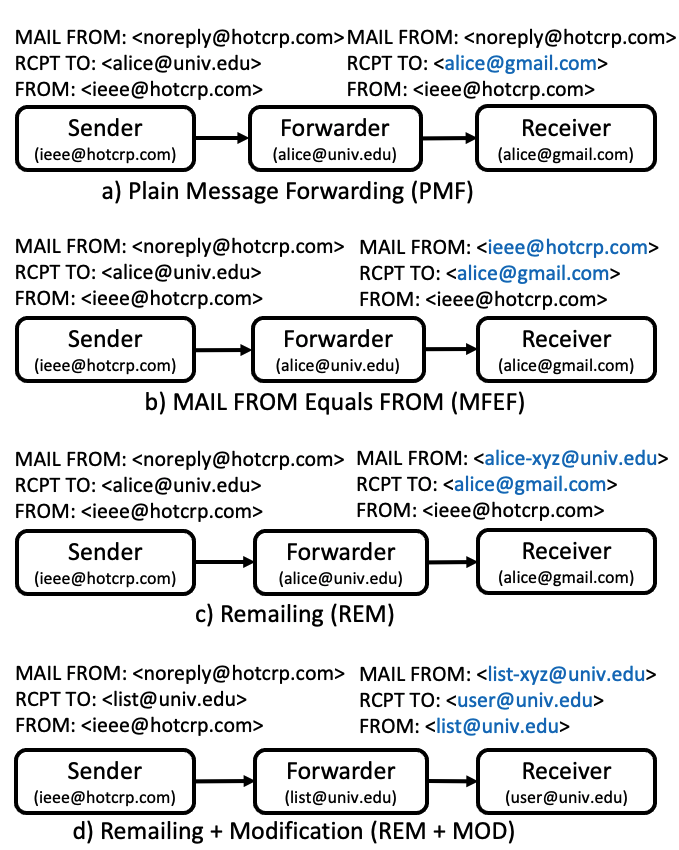
\includegraphics[width=\columnwidth]{graphs/table_forwarding_mechanisms_combined.png}
%     \caption{Four Types of Forwarding Mechanisms}
%     \label{fig:forwarding_mechs_combined}
% \end{figure}
%
% \noindent{\bf Plain Message-Forwarding (PMF)}. Initially designed for
% the purpose of ``source-routing''~\cite{Emailfor45:online}, PMF was
% one of the first forwarding mechanisms in wide use.  PMF only changes
% the \textsc{RCPT TO} header and leaves other fields
% untouched~\cite{Emailfor45:online} when forwarding.
% Figure~\ref{fig:forwarding_mechs_combined}a depicts the actions of
% such a forwarder which changes the \textsc{RCPT TO} header to the
% address of the receiver (\dns{c@c.com}) and leaves all other fields
% intact.
%
% In general, SPF disallows PMF, since this style of forwarding often
% causes SPF checks to fail at the final receiver.  Nevertheless, as we
% detail later, many email providers, like Yahoo and Fastmail, still use
% PMF in practice, which can result in security issues.
%
% {\bf Remailing (REM)}. Compared to PMF, remailing (aka redistribution),
% works well with SPF. It refers to re-sending a message and also
% rewriting the \textsc{MAIL FROM} field. It is commonly named remailing
% because the process resembles the action of a Mail User Agent
% submitting a new
% message\cite{SenderRe69:online}. Figure~\ref{fig:forwarding_mechs_combined}b
% depicts an example of how headers are modified in remailing. The
% forwarder (\dns{b.com}) first changes the \textsc{RCPT TO} header
% to reflect the destination email address (\dns{c@c.com}). It also
% rewrites the \textsc{MAIL FROM} header to reflect an address in its
% own domain (e.g., \dns{xyz@b.com}).\footnote{The exact username (the
%   ``xyz'' part) in the \textsc{MAIL FROM} address after rewriting
%   depends on the specific implementation.}  The Sender Rewriting
% Scheme, defined in RFC 5231~\cite{rfc5231}, provides a generic
% framework for rewriting email addresses in the \textsc{MAIL FROM}
% header. However, in reality, providers do not strictly follow this
% scheme.
%
% While REM works for well for SPF, it is not very compatible with
% DMARC. Without a valid DKIM header, which can happen sometimes (\eg,
% mailing lists alter a user's post signed by DKIM~\cite{rfc6783}), email
% messages forwarded via REM would fail DMARC's alignment test, and thus
% DMARC authentication. This creates a problem if the \textsc{FROM}
% domain has strict DMARC policies like quarantine or reject.
%
% \noindent{\bf Remailing with Modification (REM + MOD)}. Email
% forwarded by mailing lists that exercise REM and also alter message
% content can also sometimes fail DMARC. Remailing with Modification (REM +
% MOD) was introduced to address this issue and ensures forwarded email
% messages will pass SPF and DMARC. Besides modifying the headers
% mentioned in REM, REM + MOD also rewrites the \textsc{FROM}
% header~\cite{rfc6783}.  Figure~\ref{fig:forwarding_mechs_combined}c
% shows an example of such a modification.  Here, a forwarder
% (\dns{b@b.com}) modifies \textsc{MAIL FROM} and \textsc{RCPT TO}
% headers like REM.  Additionally, it changes the \textsc{FROM} header
% to an email address in its own domain (\dns{b@b.com}).
%
% While fully compatible with DMARC, for the same reason REM + MOD also
% introduces new security concerns. A spoofed email forwarded via REM +
% MOD is ``laundered'' with a new set of headers that will always pass
% SPF and DMARC checks, making it no different than other legitimate
% email messages.
%
%
% \noindent{\bf MAIL FROM Equals From (MFEF)}. Unlike the three
% forwarding mechanisms described above, for which we can find some
% public documentation, MAIL FROM Equals From is a custom forwarding
% mechanism that appears to only be used by Outlook.\footnote{We are not
%   entirely clear what function MFEF serves but we hope, as part of our
%   disclosure interactions with Microsoft, to gain a better
%   understanding of this design's motivation for a future version of
%   this paper.}  An example of MFEF is shown in
% Figure~\ref{fig:forwarding_mechs_combined}d.  In addition to rewriting
% the \textsc{RCPT TO} header to reflect the final receiver
% (\dns{c@c.com}), the forwarder also sets the \textsc{MAIL FROM}
% header to be the same as the \textsc{FROM} header (\dns{a@a.com}),
% regardless of the original \textsc{MAIL FROM} header
% (\dns{z@a.com}). In many scenarios, like PMF, MFEF also will break
% SPF.
%
% %\subsection{Authenticating Email Forwarding}
% %\gakiwate{Can this be confused with simple email forwarding. fwd:
% %  kind?}  As we previously discussed, email authentication using SPF,
% %DKIM and DMARC may lead to email deliverability issues. Thus,
% %forwarders may modify email headers before forwarding to ensure the
% %authentication checks still work.  As such, the receiver implicitly
% %relies on the intermediate forwarders to authenticate the email before
% %modifying it and sending it along.  However, as we demonstrate
% %(Section~\ref{sec:vulnerabilities_in_the_wild}) these assumptions may
% %not always
%
% %For example, an adversary could coax a
% %legitimate forwarder to forward a spoofed email by manually whitelisting domains
% %(Section~\ref{subsec:attack_open_forwarding}). Perhaps more egregiously, some
% %forwarders do not enforce DMARC and forward every email they receive
% %(Section~\ref{subsec:vul:no_dmarc}). Moreover, even the receiver could
% %incorrectly handle the authentication of forwarded emails
%
% \subsection{Authenticated Received Chain}
% \label{sec:arc}
%
% Given the limitations of SPF, DKIM, and DMARC in the presence of
% forwarding, a new mechanism called Authenticated Received Chain
% (ARC)~\cite{rfc8617} was recently introduced to preserve email
% authentication results across multiple forwarders.  ARC chains enable
% a receiver, who might otherwise discard a message, to evaluate the
% full set of intermediary forwarders involved in transmitting the email
% in order to make appropriate exceptions and allow legitimately
% forwarded messages to be delivered~\cite{ARCSpeci1:online}.
%
% %ARC was proposed to solve the deliverability issue introduced by forwarding.
% Intermediary hops implementing ARC sign their authentication results
% (using ARC specific headers) so that these results are accessible by the
% receiver. The expectation is that, in the case where DMARC authentication fails,
% if an ARC chain is present
% %and validated,
% a receiver might choose to
% evaluate the ARC results and allow legitimate emails to be delivered.
%
% However, ARC is currently an experimental standard and only
% implemented by a few providers~\cite{rfc8617, ARCSpeci1:online}. Among
% these, many providers maintain a list of trusted forwarders that
% implement ARC~\cite{Senderau57:online} instead of trusting all
% ARC forwarders. However, any such trust implicitly
% assumes that those trusted forwarders have good security practices.
% Unfortunately, as we detail later, this is not always the case, which
% creates additional opportunities for adversaries
% (Section~\ref{subsec:attack_zoho_arc}).

\subsection{Related Work}

Email security has been a long-standing problem and a variety of prior research efforts have examined different aspects of it. One line of work focuses on understanding and defending against phishing attacks. This includes papers that design new tools for detecting both traditional phishing and sophisticated spearphishing attacks~\cite{abu2007comparison,bergholz2008improved, fette2007learning, garera2007framework, whittaker2010large, duman2016emailprofiler, khonji2011mitigation, zhao2016optimizing, stringhini2015ain, ho19, ho17, cidon19},
study the characteristics of real-world phishing attacks~\cite{han2016phisheye,onaolapo2016happens,thomas2014consequences,bursztein2014handcrafted}, and examine the human aspect of such attacks~\cite{lastdrager2017effective, reinheimer2020investigation,abu2007comparison,
mayer2022don,caputo2013going,
Spero20, Sheng10, Kumaraguru10}.

Another body of work investigates the security and deployment of email encryption mechanisms, such as PGP~\cite{muller2019johnny, poddebniak2018efail, schwenk2020mitigation, muller2020mailto,stransky202227}, DANE~\cite{lee2022under,lee2020longitudinal}, and STARTTLS~\cite{zakir15,Foster15,poddebniak2021tls,holz2015tls,mayer2016no}.

A third research direction analyzes the security and deployment of anti-spoofing protocols such as SPF, DKIM and DMARC, with efforts from both industry and academia. The blogposts by Ullrich~\cite{Breaking12:online} and Haddouche~\cite{Mailsplo10:online} investigated approaches for bypassing DKIM and DMARC using malformed email messages.
Other work has empirically measured the efficacy and deployment status of SPF, DKIM, and DMARC~\cite{hu_end--end_nodate, zakir15, Foster15, tatang2021evolution, deccio21, wang2022large, bennett2022spfail}, as well as qualitatively characterized the factors that drive DMARC policy decisions~\cite{hutowardsunderstanding}.
% systematically researched the deployment of SPF, DKIM and DMARC, including
% the empirical study by Hu \etal\ of anti-spoofing efficacy among
% providers, a subsequent qualitative study
% to investigate the
% factors that
% drive DMARC policy decisions~\cite{hutowardsunderstanding}, and empirical measurement studies of the deployment of SPF, DKIM and DMARC by Durumeric et al.~\cite{zakir15}, Foster et al.~\cite{Foster15}, Tatang et al.~\cite{tatang2021evolution}, Deccio et al.~\cite{deccio21} and Wang et al.~\cite{wang2022large}.

The work most related to our own includes Chen et al.'s analysis of
the security vulnerabilities introduced by protocol composition in
modern email delivery~\cite{chen2020composition}, Shen et al.'s
analysis~\cite{shen2020weak} of modern sender spoofing attacks, and Wang et al.'s~\cite{wang2022revisiting} analysis of email security under the experimental Authenticated Received Chain (ARC) protocol~\cite{rfc8617}.
Of these, Chen et al.~\cite{chen2020composition} do not consider forwarding at all and Wang et al.~\cite{wang2022revisiting} focus on ARC and only consider one specific forwarding implementation as well (REM+MOD in Section~\ref{sec:measure_forwarding_mechs_and_arc}), leaving many other vulnerable forwarding mechanisms and features unexplored.

Shen et al.'s work~\cite{shen2020weak} is the closest in that it also
examines open forwarding, but because they only consider one
forwarding mechanism (what we label as REM in
Section~\ref{sec:measure_forwarding_mechs_and_arc}), they do not
identify the significant scope of this issue.  We build on and
generalize this work to show, among other attacks, that attackers are
able to practically abuse open forwarding to spoof \emph{any} domain
that includes the forwarding domain's SPF record in their own SPF record (a
common practice when hosting email via Microsoft's Outlook service for example).

% and does not illuminate many of the attacks described in our work.
% in Section~\ref{subsec:attack_open_forwarding}

%Additionally, we show how a bug they disclosed in Zoho's ARC implementation, they did not demonstrate how to use this vulnerability in practical attacks.
% due to their limited scope
%In contrast, we present a viable attack that allows an adversary to deliver spoofed email messages addressed from arbitrary domains to arbitrary Zoho users (Section~\ref{subsec:attack_zoho_arc}).
% Similarly, while they were the first to disclose Zoho's buggy ARC implementation, they missed the attack we describe in Section~\ref{subsec:attack_zoho_arc} due to limited scope --- that they only examined ARC in the context of Gmail and Zoho and did not consider forwarding configurations, which are critical components that enable the attack.

In summary, our work builds on the insights of prior efforts, but focuses exclusively and deeply on the particular security challenges introduced by the design and features of common forwarding mechanisms, and their complex interactions with existing email protocols. Through systematic measurements and analysis, we not only show that prior work largely underestimates the risks of open forwarding,
% (Section~\ref{subsec:attack_open_forwarding}),
but also reveal new attacks not discovered in prior work.
%(Section~\ref{sec:attacks}).



%Since
%forwarding is not the main focus of Shen et al.~\cite{shen2020weak},
%they only present a limited set of results: (1) their forwarding
%mechanism is limited to REM, understating many of the potential
%security issues (2) They examine open forwarding in the context of
%REM, (3) they do not elaborate on capacity of attacks introduced by
%certain vulnerabilities (\eg, the Zoho bug). (4) their work is limited
%to mail providers. In comparison, our work: (1) performs a systematic
%and empirical analysis of forwarding mechanisms used in wild,
%discovering three other broad types of forwarding mechanisms (2)
%Comprehensively measures vulnerabilities exist at all parties involved
%in the email forwarding flow \alex{we omit vulnerabilities they
%  discovered but not used in our attacks} (3) Uncovers security issues
%associated with certain vulnerabilities that are understated (\eg,
%open forwarding and Zoho's ARC bug). Our work also leads to a patch of
%the ARC bug by Zoho (\S~\ref{sec:disclosure}). (4) We also consider
%security issues centered around another common use case of forwarding
%--- mailing lists.

%Besides~\cite{shen2020weak}, other work has talked about different
%ways of bypassing email security protocols. For example,

%\alex{Phishing citations cam be added later}

